\documentclass[11pt]{article}
\usepackage[utf8]{inputenc}
\usepackage[english]{babel}
\usepackage{amsmath}
\usepackage{graphicx}
\usepackage{float}
\usepackage{lipsum}
\usepackage{multicol}
\usepackage{xcolor}
\usepackage{tabularx}
\usepackage{booktabs}
\usepackage{hyperref}
\newcolumntype{Y}{>{\centering\arraybackslash}X}
\usepackage[left=2.00cm, right=2.00cm, top=2.00cm, bottom=2.00cm]{geometry}
\usepackage{enumitem}

\title{AN2DL Reports Template}

\begin{document}

\begin{figure}[H]
      \raggedright
      
\includegraphics[scale=0.4]{polimi.png} \hfill
      
\includegraphics[scale=0.3]{airlab.jpeg}
\end{figure}

\vspace{5mm}

\begin{center}
      % Select between First and Second
      {\Large \textbf{AN2DL - First Homework Report}}\\
      \vspace{2mm}
      % Change with your Team Name
      {\Large \textbf{LosPollosHermanos}}\\
      \vspace{2mm}
      % Team Members Information
      {\large Mohammadhossein Allahakbari,}
      {\large Michele Miotti,}
      {\large Francesco Pesce}\\
      \vspace{2mm}
      % Codabench Nicknames
      {mh2033,}
      {michelem,}
      {francescopesce}\\
      \vspace{2mm}
      % Matriculation Numbers
      {246639,}
      {249499,}
      {247974}\\
      \vspace{5mm}
      \today
\end{center}
\vspace{5mm}

\begin{multicols}{2}
      % Note: The following sections represent a suggested
      % structure. We don't need to follow it strictly.

      % -----------------------------------------------------------------------
      % INTRODUCTION
      % -----------------------------------------------------------------------
      \section{Introduction}
      % In this section, you should present your project's context and
      % objectives. You might want to:
      % \begin{itemize}
      %     \item Dehe problem (\textit{you may use italics to highlight
      %               definitions})
      %     \item State your goals (\textbf{emphasise key points with bold})
      %     \item Outline your approach
      % \end{itemize}

      % \noindent For instance, you might write: ``This project focuses on
      % \textit{image classification} using \textbf{deep learning} techniques."

      This report presents the results of the \textit{image classification}
      task proposed in the first homework of the \texttt{Artificial Neural Networks and Deep Learning} course at Politecnico di Milano. The goal of the project is to classify blood cell images into 8 different classes by using deep learning techniques such as \textit{Convolutional Neural Networks} (CNNs)\cite{NIPS1989_53c3bce6}.

      % -----------------------------------------------------------------------
      % PROBLEM ANALYSIS
      % -----------------------------------------------------------------------
      \section{Problem Analysis}
      % Here you can discuss your initial analysis of the problem. Consider
      % including:
      % \begin{enumerate}
      %     % 8 classes, 96x96 rgb images, labels, etc
      %     \item Dataset characteristics
      %     \item Main challenges % The test set is horrible
      %     That the test set was not horrible? Is this what they mean?
      %     \item Initial assumptions 
      % \end{enumerate}

      % \noindent If you need to reference papers, use the citation command:
      % Recent work~\cite{lecun2015deep} suggests..."

      The task involved the use of three datasets, only one of which was available to us. The others were used by the Codabench\cite{codabench} platform to evaluate the developed models, with different datasets used in the Development and Final phases.

      The provided dataset consisted in around 10,000 RGB images of blood cells, each of size 96\(\times\)96 pixels, to be classified into 8 different categories. We modeled the problem as a \textit{multi-label classification} problem, where each image is an observation of a random variable with an unknown distribution.
      
      After manually analyzing the dataset, we found that it contained some very clear outliers, i.e. duplicate and misleading images that were doctored by adding unrelated overlays. As such, we decided to remove said images from the dataset.

      Furthermore, after testing our first model on a local test set, we found that the model's performance on the Codabench platform was significantly lower. Since the mismatch appeared with multiple models, that images in the dataset present on Codabench could not be reasonably assumed to have been generated by the same distribution that generated the images we were provided, and were likely doctored in some way.

      The samples of different labels in the dataset was moderately imbalanced. Using data augmentation techniques to balance out the number of samples for each class in the training set seemed to indicate that the distribution of labels in the closed datasets was the same as in the provided one. As such, there was no need to adjust the prior distribution of the labels.

      % -----------------------------------------------------------------------   
      % METHOD
      % -----------------------------------------------------------------------
      \section{Method}
      % Not sure what they are asking here. The final model?
      % This section should detail your approach. You can use equations to
      % explain your methodology. For example, a simple model representation:
      % \begin{equation}
      %     \label{eq:model}
      %     f(x) = \text{softmax}(Wx + b)
      % \end{equation}

      % \noindent Or a more complex loss function:
      % \begin{equation}
      %     \label{eq:loss}
      %     \mathcal{L} = -\frac{1}{N}\sum_{i=1}^{N} y_i\log(\hat{y}_i)
      % \end{equation}

      % \noindent Reference these equations in your text, like:``As shown in
      % equation~\ref{eq:model}..."

      Most of the development process was done on a \texttt{Jupyter} notebook, using the \texttt{Tensorflow}\cite{TensorFlow} and \texttt{Keras}\cite{Keras} libraries for \texttt{Python}, mostly run locally, due to strict GPU usage limits of popular platforms, such as \texttt{Google Colab}.

      We initially split our dataset into training, validation and test sets, but upon noticing that the accuracy on the local test set was unrelated to the accuracy on Codabench, we decided to get rid of it, and apply an 80-20 training-validation split.

      All developed models contain a convolutional CNN core, due to two of their properties: \textit{automatic feature extraction} and \textit{sparsity} of the weights with respect to dense neural networks, fundamental properties when the inputs are images. The latent representation is then used by a dense neural network, with 8 output neurons and a softmax activation. Since this is a multi-class classification problem, the loss function we employed was categorical crossentropy, as minimizing said loss function maximizes the likelihood of generating the data\cite{shalev2014understanding}.

      After experimenting with diverse techniques, as detailed in Section \ref{sec:experiments}, we found that the best approach was to use a chain of two convolutional and downsampling layers, followed by two instances of a custom block, illustrated in Section \ref{sec:custom_block}. The output of these custom blocks is then fed into a \texttt{Global Average Pooling}\cite{Lin2013NetworkIN} layer, used as a structural regularizer. The dense network at the top of the net has a hidden layer, followed by a \texttt{Dropout} layer for regularization, and \texttt{Batch Normalization}\cite{pmlr-v37-ioffe15} is performed after each convolutional layer. The model was trained using the \texttt{Adam}\cite{Kingma2014AdamAM} optimizer with early stopping after 40 epochs of stagnation of validation accuracy, 1e-3 initial learning rate and adaptively lowering the learning rate 5-fold after 20 epochs of stagnation in validation loss.

      The final network has 1.9 million parameters, achieved an accuracy of 88.5\% on the final dataset on Codabench, and was developed after exploring a complex design space formed by the number of custom and convolutional blocks, presence of the hidden dense layer, optimizer used, learning rate and other variables.

      % -----------------------------------------------------------------------
      % EXPERIMENTS
      % -----------------------------------------------------------------------
      \label{sec:experiments}
      \section{Experiments}
      % Step 1: bad CNN just to test things out
      % Step 2: normal augmentation
      % Step 3: overlaying
      % Step 4: keras cv (gigachad picture)
      % Step 5: testing residual networks (up to 0.8)
      %   and inception blocks (up to 0.72)
      % Step 6: custom block (in detail)
      % Step 7: add more filters
      % Step 8.....: not done yet
      % If you need accuracies, number of parameters etc ask me

      % Failed experiments:
      % transfer learning (bad accuracy) (VGG, MobileNet, ResNet), both with and
      % without fine tuning
      % Lion, stochastic gradient descent with momentum

      % Ideas that worked momentarily:
      % voting mechanism with multiple neural networks
      % averaging weights below a certain validation loss
      We performed many experiments, some of which significantly improved the accuracy of our models. In chronological order, the main breakthroughs were:
      \begin{itemize}[leftmargin=*]
            \setlength\itemsep{0em}
            \item \textbf{Simple CNN:} A simple CNN was developed to test the development flow and the platform, making us realize that the Codabench dataset was likely doctored in some way.
            \item \textbf{Data Augmentation:} We implemented simple image augmentation techniques.
            \item \textbf{Overlaying:} After finding the outliers in the dataset, we hypothesized that the test set may have been doctored in the same way, so we experimented with applying overlays to the images in our dataset, using techniques such as convex combinations and multiplicative overlays.
            \item \textbf{Keras CV:} Using the \texttt{KerasCV} library\cite{chollet2015keras} provided the first satisfactory results. The library provides richer augmentations, which can be applied in a complex pipeline. Since they are applied during training, augmentations can use different seeds at different epochs, fully utilizing the information in the training set. The overlaying technique was removed due to poor compatibility, and both the training and validation sets we augmented, since images on Codabench were likely more "similar" to augmented ones.
            \item \textbf{Richer models:} We experimented with \texttt{In\-cep\-tion} blocks\cite{Inception}, \texttt{Re\-si\-dual net\-works}\cite{He2015DeepRL}, \texttt{Glo\-bal Aver\-age Poo\-ling} and \texttt{Batch Nor\-ma\-li\-za\-tion} layers.
            \item \textbf{Custom Block:} A custom block was implemented to mix the features of \texttt{Re\-si\-dual} and \texttt{In\-cep\-tion} blocks. The rationale and more details are discussed in section \ref{sec:custom_block}.
      \end{itemize}

      We also performed experiments with less fortunate results. One that merits explicit mention is using \textit{transfer learning}\cite{TransferLearning} from some well-known CNN architectures, such as \texttt{VGG19}, \texttt{ResNet50V2} and \texttt{MobileNetV2}, using the \textit{ImageNet}\cite{ImageNet} pre-trained weights, with a custom dense network. We attempted both training just the latter and unfreezing the top convolutional layers, but achieved very poor results with both techniques. These results, the large memory requirements of the models, problematic for both local training and the Codabench platform, and the wish to create our own custom model, led us to abandon this avenue. Other failed experiments include using the \texttt{Lion} and \texttt{SGD} with momentum optimiers provided by \texttt{Keras} in place of \texttt{Adam}, performing test-time augmentations, attempting to filter out noise in test images using Fourier transforms and filters, and mixed precision.

      Other ideas were successful at first, such as averaging weights from all epochs below a certain validation loss as a regularization technique, and a voting mechanism with CNNs, acting as a sort of \textit{ensemble} method. The ideas were effective on early models, but did not have an effect on more fine-tuned ones.

      % For your experiments, you might want to present your results in tables.
      % Here's an example of a wide table comparing different models:

      % \begin{table*}[t]
      %     \centering
      %     \setlength{\tabcolsep}{3pt}
      %     \caption{An example of wide table. Best results are highlighted in
      %         \textbf{bold}.}
      %     \begin{tabularx}{\textwidth}{lYYYc}
      %         \toprule
      %         Model            & Accuracy                  & Precision
      %                          & Recall                    & ROC AUC
      %         \\
      %         \midrule
      %         VGG18            & 72.20 $\pm$ 3.06          & 94.95 $\pm$ 0.52
      %                          &
      %         86.95 $\pm$ 0.55 & 80.16 $\pm$ 0.81
      %         \\
      %         Custom Model     & 27.71 $\pm$ 3.19          & 75.70 $\pm$ 1.07
      %                          & 55.75 $\pm$ 2.16          & 36.60 $\pm$ 1.26
      %         \\
      %         ResNet18         & \textbf{89.24 $\pm$ 2.38} & \textbf{95.54
      %         $\pm$ 0.49}      & \textbf{93.43 $\pm$ 1.30} & \textbf{91.68 $\pm$
      %             0.71}
      %         \\
      %         \bottomrule
      %     \end{tabularx}
      %     \label{tab:Performance}
      % \end{table*}

      % \noindent For more specific measurements, you might use a narrower
      % table:

      % \begin{table}[H]
      %     \centering
      %     \setlength{\tabcolsep}{3pt}
      %     \caption{An example of table. Best results may be highlighted in
      %         \textbf{bold}.}
      %     \begin{tabularx}{\linewidth}{lY}
      %         \toprule
      %         Time [$\mu$s] & Distance [mm] \\
      %         \midrule
      %         22$\pm$4      & 8$\pm$1       \\
      %         17$\pm$3      & 7$\pm$1       \\
      %         15$\pm$3      & 6$\pm$1       \\
      %         13$\pm$2      & 5$\pm$1       \\
      %         10$\pm$2      & 4$\pm$1       \\
      %         8$\pm$2       & 3$\pm$1       \\
      %         5$\pm$1       & 2$\pm$1       \\
      %         37$\pm$1      & 1$\pm$1       \\
      %         \bottomrule
      %     \end{tabularx}
      %     \label{tb:Measurements}
      % \end{table}

      % \noindent You can also include figures to visualise your results:
      % \begin{figure}[H]
      %     \centering
      %     
\includegraphics[width=0.75\linewidth]{random.jpeg}
      %     \caption{Example figure showing [describe what the figure shows]}
      %     \label{fig:results}
      % \end{figure}

      % \noindent Reference figures using like:``As shown in
      % Figure~\ref{fig:results}..."

      % -----------------------------------------------------------------------
      % CUSTOM BLOCK
      % -----------------------------------------------------------------------
      \label{sec:custom_block}
      \section{Custom Block}
      % Explain the custom block in detail

      \begin{figure}[H]
            \centering
            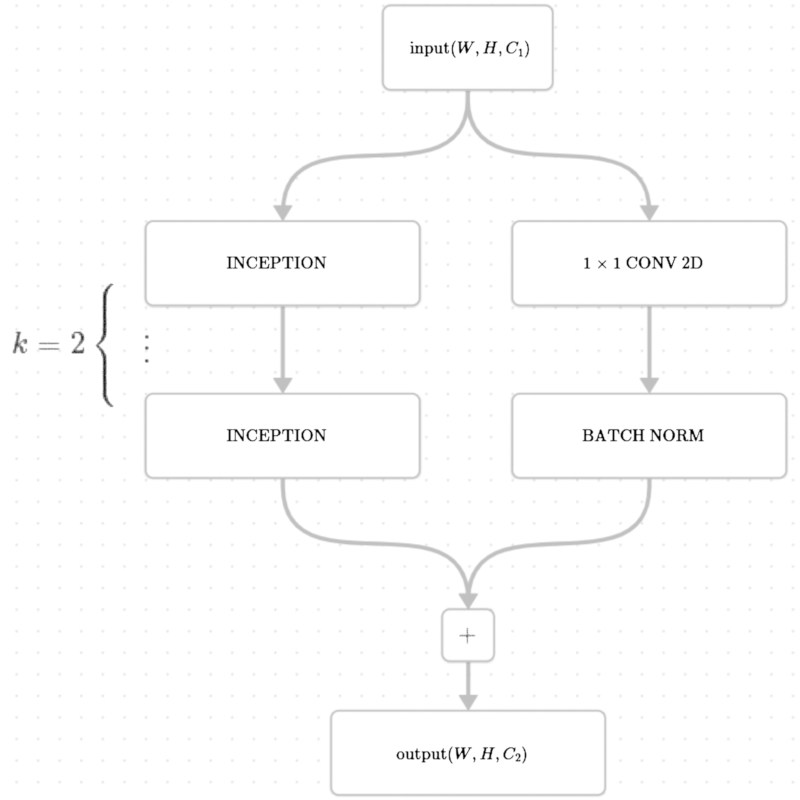
\includegraphics[width=0.75\linewidth]{custom_block.png}
            \caption{The structure of our custom block.}
            \label{fig:custom_block}
      \end{figure}

      In 2015, \texttt{ResNet} revolutionized CNNs by injecting skip connections into the network, which help the learning process by making deeper levers learn residuals with respect to the identity function. Adding said connections to a simple CNN design significantly improved the accuracy of our models, up to 0.8 on Codabench.

      In \texttt{Inception} blocks, a set of differently sized filters are applied to the block's input, and the results are concatenated as output channels. Adding \texttt{Inception} blocks our design did not improve our accuracy. However, as opposed to previous experiments, were each model classified correctly most of the same images as its predecessors plus some more, networks containing just simple \texttt{Residual} and just \texttt{Inception} blocks were able to correctly classify different images. This led us to hypothesize that the models captured different features of the dataset, and could be combined to improve the accuracy even further. By combining the two blocks, we created what, to the best of our knowledge, is a new block. It is formed by stacking a certain number \texttt{k} of \texttt{Inception} blocks, and then introducing a skip connection, as shown in Figure \ref{fig:custom_block}.

      % -----------------------------------------------------------------------
      % RESULTS
      % -----------------------------------------------------------------------
      \label{sec:results}
      \section{Results}
      % Keras CV is good
      % Combining residual and inception is good
      % Present your main findings here. You might want to:
      % \begin{itemize}
      %     \item Compare your results with baselines
      %     \item Highlight key achievements using \textbf{bold text}
      %     \item Explain any unexpected outcomes
      % \end{itemize}

      During the Development phase, we trained and submitted more than 50 models. Table \ref{tab:results} shows the best result using each of the techniques discussed in Section \ref{sec:experiments}, before introducing the next technique.

      \begin{table}[H]
          \centering
          \setlength{\tabcolsep}{3pt}
          \begin{tabularx}{\linewidth}{lY}
              \toprule
              Experiment & Accuracy \\
              \midrule
              Simple CNN & 0.20* \\
              Data Augmentation & 0.25* \\
              Overlaying & 0.53\;\, \\
              KerasCV & 0.71\;\, \\
              Richer models & 0.80\;\, \\
              Custom Block & 0.88\;\, \\
              \bottomrule
          \end{tabularx}
          \caption{Results for each technique. Results marked with * are approximate, due to being obtained before the first reset to the Codabench platform.}
          \label{tab:results}
      \end{table}

      % -----------------------------------------------------------------------
      % DISCUSSION
      % -----------------------------------------------------------------------
      \section{Discussion}
      % Wait until we have the final results
      % In this section, analyse your results critically. Consider:
      % \begin{itemize}
      %     \item Strengths and weaknesses
      %     \item Limitations and assumptions
      % \end{itemize}

      Due to the heavy usage of \textit{augmentation} and \textit{regularization} techniques, the model generalizes well the information learned from the training set. While some larger models, such as ones obtained by \textit{transfer learning}, if trained properly, may have been able to capture more features of the images and achieve higher accuracies, our model can be trained and fine-tuned on commodity hardware, has lower memory requirements and faster predictions. Moreover, we propose a \textit{scaling} technique for devices with lower capabilites. By simply substituting one of the custom blocks with a convolutional layer, and reducing the number of filters in each block, a lighter model with less than 1/10-th of the parameters can be obtained, with a respectable 0.82 accuracy on Codabench. 

      % -----------------------------------------------------------------------
      % CONTRIBUTIONS
      % -----------------------------------------------------------------------
      \section{Contributions}

      Most ideas and propositions were evenly distributed among the team members, while actual coding was more specific to each member's strengths. Many different branches were created in the project's repository to experiment with different ideas and techniques, and the final model was a result of combining the best experiments from each branch.

      % -----------------------------------------------------------------------
      % CONCLUSIONS
      % -----------------------------------------------------------------------
      \section{Conclusions}
      % Summarise your work and discuss potential future directions. This is
      % where you can:
      % \begin{itemize}
      %     \item Restate main contributions
      %     \item Suggest improvements
      %     \item Propose future work
      % \end{itemize}

      In this project, we developed and trained a custom CNN, using techniques from CNNs in the scientific literature. The model achieved an accuracy of 88.4\% on the final dataset on the Codabench platform, and makes use of a custom block we developed by reasoning about the properties of the blocks we were shown in class. Future work could include a more thorough analysis of the design space for the model, especially when it comes to the specific augmentation techniques, which seem to have a large effect on accuracy, and further attempts at transfer learning, which, if successful, could result in a detailed comparison between our custom model and said models. Overall, the project's challenge-like nature helped us follow a structured approach to solving the problem. The lack of a pristine test set gave us the opportunity to test out many different techniques and apply what was taught in class, instead of quickly finding a satisfactory result. 

      % Remember to include the bibliography!
      \bibliography{references}
      \bibliographystyle{abbrv}

\end{multicols}
\end{document}